\section{eo\-VRPOne\-Point\-Crossover Class Reference}
\label{classeo_v_r_p_one_point_crossover}\index{eoVRPOnePointCrossover@{eoVRPOnePointCrossover}}
Implementation of the simple One Point Crossover.  


{\tt \#include $<$eo\-VRPQuad\-Crossover.h$>$}

Inheritance diagram for eo\-VRPOne\-Point\-Crossover::\begin{figure}[H]
\begin{center}
\leavevmode
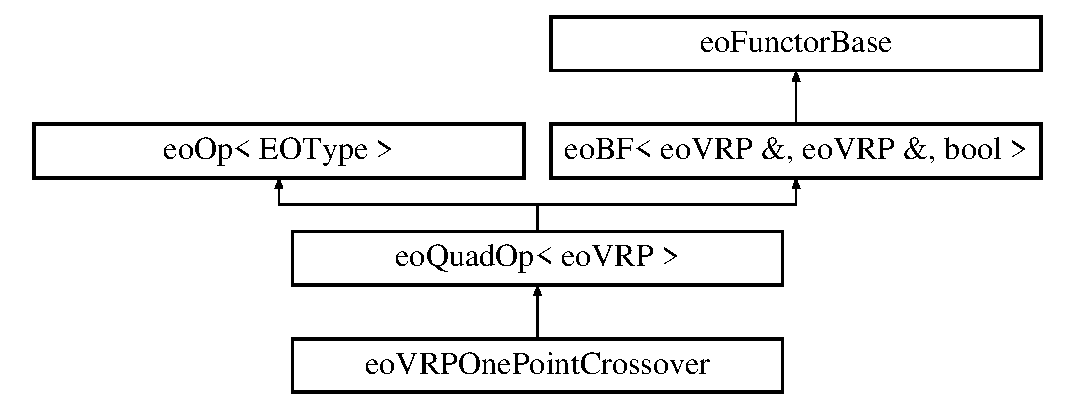
\includegraphics[height=4cm]{classeo_v_r_p_one_point_crossover}
\end{center}
\end{figure}
\subsection*{Public Member Functions}
\begin{CompactItemize}
\item 
\bf{eo\-VRPOne\-Point\-Crossover} ()\label{classeo_v_r_p_one_point_crossover_24f40efc1adb60947c5d533653bbfbe9}

\begin{CompactList}\small\item\em Deafult constructor. \item\end{CompactList}\item 
std::string \bf{class\-Name} () const 
\begin{CompactList}\small\item\em Returns a string containing the name of the class. \item\end{CompactList}\item 
bool \bf{operator()} (\bf{eo\-VRP} \&\_\-genotype1, \bf{eo\-VRP} \&\_\-genotype2)
\begin{CompactList}\small\item\em Performs a one point crossover. \item\end{CompactList}\end{CompactItemize}


\subsection{Detailed Description}
Implementation of the simple One Point Crossover. 



Definition at line 159 of file eo\-VRPQuad\-Crossover.h.

\subsection{Member Function Documentation}
\index{eoVRPOnePointCrossover@{eo\-VRPOne\-Point\-Crossover}!className@{className}}
\index{className@{className}!eoVRPOnePointCrossover@{eo\-VRPOne\-Point\-Crossover}}
\subsubsection{\setlength{\rightskip}{0pt plus 5cm}std::string eo\-VRPOne\-Point\-Crossover::class\-Name (void) const\hspace{0.3cm}{\tt  [inline, virtual]}}\label{classeo_v_r_p_one_point_crossover_a62bc52e6f36d7fae7c192173fbfd2dc}


Returns a string containing the name of the class. 

Used to display statistics. \begin{Desc}
\item[Returns:]The string containing the name of the class. \end{Desc}


Reimplemented from \bf{eo\-Quad\-Op$<$ eo\-VRP $>$}.

Definition at line 177 of file eo\-VRPQuad\-Crossover.h.\index{eoVRPOnePointCrossover@{eo\-VRPOne\-Point\-Crossover}!operator()@{operator()}}
\index{operator()@{operator()}!eoVRPOnePointCrossover@{eo\-VRPOne\-Point\-Crossover}}
\subsubsection{\setlength{\rightskip}{0pt plus 5cm}bool eo\-VRPOne\-Point\-Crossover::operator() (\bf{eo\-VRP} \& {\em \_\-genotype1}, \bf{eo\-VRP} \& {\em \_\-genotype2})\hspace{0.3cm}{\tt  [inline, virtual]}}\label{classeo_v_r_p_one_point_crossover_b930b5d9a8ee0719f675f9eea791579b}


Performs a one point crossover. 

Both parameters are the parents and the (future) children of the crossover. \begin{Desc}
\item[Parameters:]
\begin{description}
\item[{\em \_\-genotype1}]The first parent. \item[{\em \_\-genotype2}]The second parent. \end{description}
\end{Desc}
\begin{Desc}
\item[Returns:]True if any of the parents was modified. False otherwise. \end{Desc}


Implements \bf{eo\-BF$<$ eo\-VRP \&, eo\-VRP \&, bool $>$}.

Definition at line 191 of file eo\-VRPQuad\-Crossover.h.

References eo\-VRP::clean\-Routes(), and eo\-Rng::random().

The documentation for this class was generated from the following file:\begin{CompactItemize}
\item 
eo\-VRPQuad\-Crossover.h\end{CompactItemize}
